\documentclass[UTF8]{ctexrep} % Chinese language class type, need XeLaTeX to compile
\usepackage{hologo} % needed for reference
\usepackage{gbt7714} % needed for reference
\usepackage{float} % needed for [H] strick floating option
\usepackage{caption} % needed for command \captionsetup in longlisting new environment
\usepackage{subcaption} % needed for command \captionsetup in longlisting new environment
\usepackage{graphicx} % needed for displaying eps file
\usepackage{longtable} % to display tables on several pages
\usepackage{rotating} % to display tables in landscape
\usepackage{multirow} % for multirow tables
\usepackage{booktabs} % for prettier tables
\usepackage[title]{appendix} % create appendices
%-----------------------------------------------------------------------------------------
% To write pseudo-code
%-----------------------------------------------------------------------------------------
\usepackage{algorithm}  
\usepackage{algpseudocode}
\usepackage{amsmath}
\usepackage{amssymb}
\renewcommand{\algorithmicrequire}{\textbf{Input:}}  % Use Input in the format of Algorithm  
\renewcommand{\algorithmicensure}{\textbf{Output:}} % Use Output in the format of Algorithm
%-----------------------------------------------------------------------------------------
% To adjust geometry and stuff
%-----------------------------------------------------------------------------------------
\usepackage{geometry} % adjust margin and what
\geometry{a4paper} % use A4 paper to make the report look good enough
%-----------------------------------------------------------------------------------------
% To define colors yourself
%-----------------------------------------------------------------------------------------
\usepackage{xcolor} % needed for defining own color
\definecolor{myred}{RGB}{223, 56, 27}
\definecolor{myblue}{RGB}{25, 123, 193}
\definecolor{myorange}{RGB}{225, 107, 65}
\definecolor{mypink}{RGB}{254, 63, 125}
\definecolor{mycyan}{RGB}{72, 199, 240}
\definecolor{mygreen}{RGB}{0, 153, 136}
%-----------------------------------------------------------------------------------------
% To use hyper-reference and stuff
%-----------------------------------------------------------------------------------------
\usepackage{hyperref} % needed for hyperlinks
\hypersetup{ % hyper link setups, can be used else where
    colorlinks=true,
    linkcolor=blue,
    filecolor=magenta,      
    urlcolor=cyan,
    pdftitle={imageRestore},
}
%-----------------------------------------------------------------------------------------
% To list code elegantly and stuff
%-----------------------------------------------------------------------------------------
\usepackage[
    % cache=false,
    newfloat=true,
    % outputdir=./
]{minted} % needed for listing
\newenvironment{longlisting}{\captionsetup{type=listing}}{}
\setminted{
    tabsize=4,
    breaklines,
    frame=single,
    linenos,
    fontsize=\small
}


\makeatletter
\newenvironment{breakablealgorithm}
  {% \begin{breakablealgorithm}
   \begin{center}
     \refstepcounter{algorithm}% New algorithm
     \hrule height.8pt depth0pt \kern2pt% \@fs@pre for \@fs@ruled
     \renewcommand{\caption}[2][\relax]{% Make a new \caption
       {\raggedright\textbf{\ALG@name~\thealgorithm} ##2\par}%
       \ifx\relax##1\relax % #1 is \relax
         \addcontentsline{loa}{algorithm}{\protect\numberline{\thealgorithm}##2}%
       \else % #1 is not \relax
         \addcontentsline{loa}{algorithm}{\protect\numberline{\thealgorithm}##1}%
       \fi
       \kern2pt\hrule\kern2pt
     }
  }{% \end{breakablealgorithm}
     \kern2pt\hrule\relax% \@fs@post for \@fs@ruled
   \end{center}
  }
\makeatother

% \algrenewtext{For}[3]%
% {\algorithmicfor\ #1 \gets #2 \algorithmicto\ #3 \algorithmicdo}


%-----------------------------------------------------------------------------------------
% To predefine title and stuff
%-----------------------------------------------------------------------------------------
\title{数据库系统实验报告\\
  B+ Tree and Index Manager in \texttt{miniSQL} \\
  \large \texttt{miniSQL}设计中的B+树和索引管理器}

\author{
教师:孙建伶\\
姓名:徐震\\
学号:3180105504\\
邮箱:\href{3180105504@zju.edu.cn}{3180105504@zju.edu.cn}\\
电话:18888916826
}
\date{\today}

\begin{document}

\maketitle
\newpage
\tableofcontents
\newpage
\part{正文}
\chapter{实验目的}
\paragraph{\texttt{miniSQL}}
设计并实现一个精简型单用户SQL引擎(DBMS)\texttt{miniSQL},允许用户通过字符界面输入SQL 语句实现表的建立/删除;索引的建立/删除以及表记录的插入/删除/查找。
\paragraph{索引管理器}
我们负责设计的索引管理器模块主要负责数据库系统中的索引管理,提供基于B+树的索引实现并提高数据库查询/插入/删除效率。并通过提供易用接口与其他模块整合实现有效功能。
\paragraph{设计目的}
通过对\texttt{miniSQL}的设计与实现,提高学生的系统编程能力,加深对数据库系统原理的理解。
通过编程设计,加深对数据库系统的理解并深入了解B+树这一数据结构。
以模块化方式构建大型计算机软件,提高架构抽象能力并重视模块化和解耦合在软件设计中的作用。
\paragraph{功能实现}
我们将实现如下的基本索引功能:
\begin{itemize}
    \item 对单属性索引提供完整支持。
    \item 通过客制化比较函数可支持简单多属性索引。
    \item 对于表的主键自动建立B+树索引/排序数组索引。
    \item 对于声明为\texttt{unique}(唯一值)的属性可以通过SQL语句由用户指定建立/删除B+树索引。
    \item 支持除B+树以外的数据结构索引(如排序数组索引),控制接口。
    \item 基于\texttt{Exception}(异常)的错误信息传递路径。
    \item 基于\texttt{Python}语言的多种数据类型索引支持。
\end{itemize}
\chapter{实验环境}
\section{系统需求}
\paragraph{主要开发语言}
\begin{itemize}
    \item Python 3.7.5
    \item Python 3.7.6
\end{itemize}
\paragraph{主要开发环境}
\begin{itemize}
    \item PyCharm 2020.1
    \item Visual Studio Code 1.45
\end{itemize}
\paragraph{经过测试的系统环境}
\begin{itemize}
    \item Microsoft Windows [Version 10.0.18363.836]
    \item Ubuntu WSL2
\end{itemize}

\section{实验环境}
\paragraph{实验系统环境} Microsoft Windows [Version 10.0.18363.836]
\paragraph{实验处理器环境} Intel(R) Core(TM) i7-9750H CPU @ 2.60GHz 12 Logical Processors
\paragraph{实验内存环境} SODIMM 15.8GB/16.0GB
\paragraph{实验硬盘环境} KBG30ZMS512G NVMe TOSHIBA 512GB

\chapter{模块设计}
\section{功能描述}
\subsection{建立/删除索引}
实际的数据库应用中,有在建立表时创建索引和表中有数据情况下创建索引的需求。区别在于,前者不需要其他模块为索引管理器提供数据,仅仅需要分配一个新索引所需的内存和磁盘空间;而后者要求发出建立索引请求的模块提供相应的数据块。默认情况下我们以记录的行号作为B+树中键值对上的“值”,因此我们要求相应数据块是按照它们将来被查找的顺序提供的。
\paragraph{建立索引}
正如图\ref{fig:index_example}所示的\footnote{图\ref{fig:index_example}来源于\textit{Database System Concepts 6th Edition Abraham Silberschatz等。}}。为了方便演示,让我们用其中的第一列作为建立索引的数据集。我们会按顺序将提供的数据插入索引数据结构,因此在这一个键值对中,键为第一列数据值,如\textit{10101},而值为行号,如\textit{0}。
\begin{figure}[H]
    \centering
    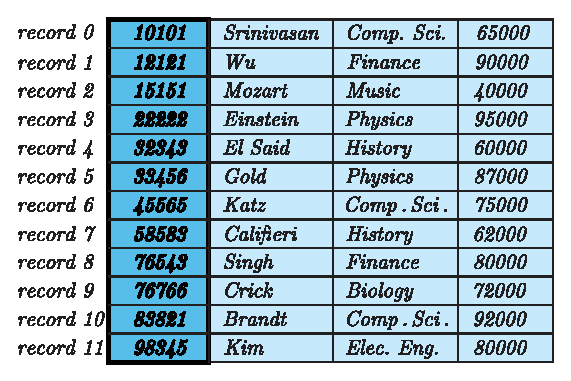
\includegraphics[width=0.7\linewidth]{figure/index_example.eps}
    \caption{线性记录储存方式}
    \label{fig:index_example}
\end{figure}

这样处理的原因在于,我们希望日后通过索引根据查找键快速找到记录对应的位置,而其在表格中的相对位置是最方便的寻址信息之一。若我们按照索引的自定义值储存插入的键,则索引失去加快搜索的作用;若我们插入的值为记录的绝对磁盘位置信息,则缓存管理器失效,且数据的移动会导致索引失效。
\par
在内存中创建索引(并插入相应数据后),索引管理器会将索引的内存信息叫给缓存管理器,由其决定是否应将内存保留或者存储到磁盘中,同时返回给索引管理器一个唯一的索引标号(索引管理器会将其继续返回给上层模块),日后将根据这一唯一标识符从缓存管理器中取得相应索引(无论是通过读取磁盘文件还是直接获取内存指针)。
\paragraph{删除索引}
我们通过上述的唯一标识符给缓存管理器发出删除信号,完成删除操作。

\subsection{查找/删除索引键}
查找和删除操作支持快速范围操作,并且两者在具体实现上有极大相似性,我们通过抽象两者的操作来提高代码复用率。
我们首先直接判断用户进行的是范围还是单值查找,并且替前从缓存管理器中取得相应索引内容(内存或硬盘中)。
\paragraph{单值操作}
我们调用B+树相应查找接口获得应查找的值,并通过异常来进行错误通讯。若查找成功则直接返回,否则抛出相关异常。
\begin{figure}[H]
    \centering
    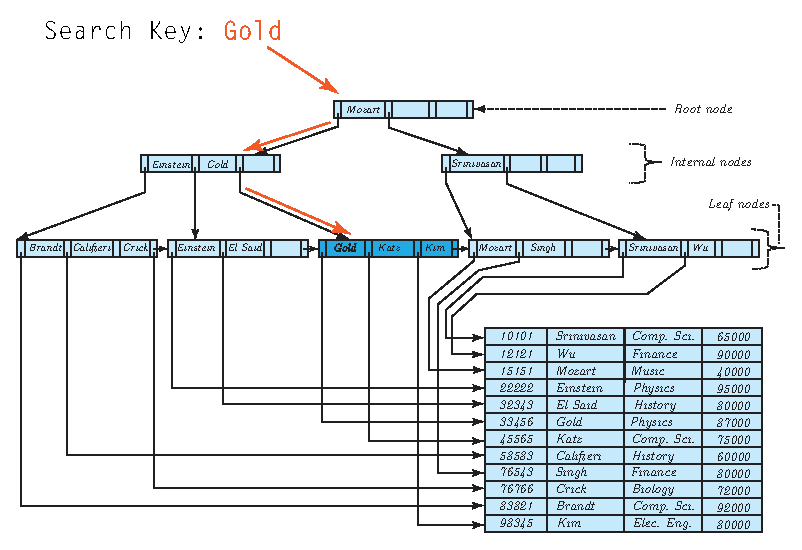
\includegraphics[width=0.75\linewidth]{figure/search_delete_single.eps}
    \caption{单值操作}
    \label{fig:search_delete_single}
\end{figure}


\paragraph{范围操作}
我们首先会检查用户给予的范围是否有效\footnote{例如,范围左右下标是否为左 小右大,或被查找的树是否为空等},同样的,我们使用异常来进行错误通讯,这使得接口模块能方便的实现错误处理。接着我们查询范围两端的值\footnote{我们默认范围查找的区间是左闭右开的。}并根据返回的节点情况进行相关操作,对于查找指令,这一操作是返回查询得到的相关信息;对于删除指令,这一操作是操作B+树删除相关的值,并在操作全部完成后将修改后的索引叫给缓存管理器。如图\ref{fig:search_delete_multi}所示(加深部分为需要查找或删除的部分)。

\begin{figure}[H]
    \centering
    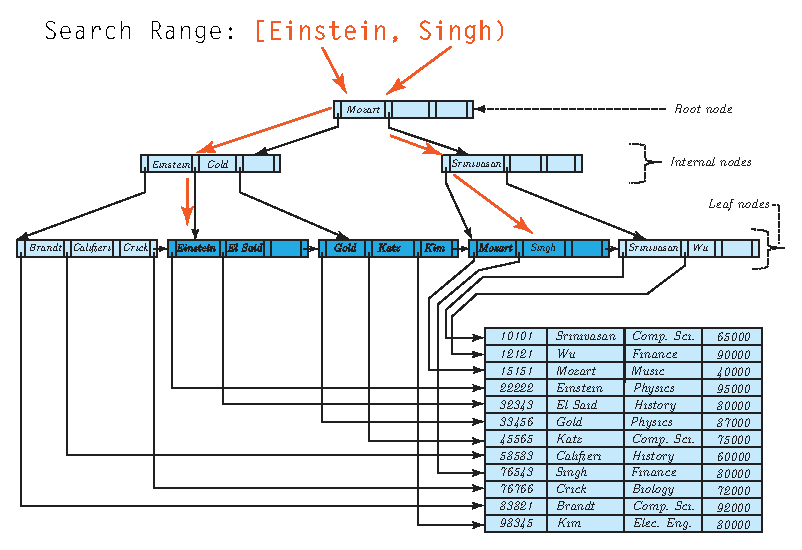
\includegraphics[width=0.75\linewidth]{figure/search_delete_multi.eps}
    \caption{范围操作}
    \label{fig:search_delete_multi}
\end{figure}

\subsection{插入键值对}
我们单独实现了插入键值对功能,因为其逻辑相对于查询和删除操作都有所不同(需检查重复元素等)。类似的,索引管理器会首先向缓存管理器请求相关索引内容。接着我们调用插入操作,将是否允许替换的信息传递给B+树的相关寒函数直接进行操作\footnote{原因在于B+树内部实现中也需要调用查找相关功能,与其规定执行流程,不如让B+树具体实现获得最优执行流程}。

\subsection{更新值内容}
由于我们使索引中键值对中\textit{值}指向记录在某张表中的位置,而这一位置在数据库运行过程中可能会发生很大变化\footnote{例如闲时的数据库清理和记录重排序等,亦或记录管理器采取了不同的数据储存模型。},我们给外界留出批量修改值的接口。
\par
这一操作类似于范围操作中涉及到的内容,我们需要对B+中的有效节点数目进行检查,根据节点数目选取不同的处理方式。

\section{主要数据结构}
\subsection{B+树}
\footnote{此段内容摘自\href{https://en.wikipedia.org/wiki/B+_tree}{WikiPedia}}
B+ 树是一种树数据结构,通常用于数据库和操作系统的文件系统中。B+ 树的特点是能够保持数据稳定有序,其插入与修改拥有较稳定的对数时间复杂度。B+ 树元素自底向上插入,这与二叉树恰好相反。
\par
B+ 树在节点访问时间远远超过节点内部访问时间的时候,比可作为替代的实现有着实在的优势。这通常在多数节点在次级存储比如硬盘中的时候出现。通过最大化在每个内部节点内的子节点的数目减少树的高度,平衡操作不经常发生,而且效率增加了。这种价值得以确立通常需要每个节点在次级存储中占据完整的磁盘块或近似的大小。
\par
B+ 背后的想法是内部节点可以有在预定范围内的可变量目的子节点。因此,B+ 树不需要像其他自平衡二叉查找树那样经常的重新平衡。对于特定的实现在子节点数目上的低和高边界是固定的。例如,在 2-3 B 树(常简称为2-3 树)中,每个内部节点只可能有 2 或 3 个子节点。如果节点有无效数目的子节点则被当作处于违规状态。
\par
B+ 树的创造者 Rudolf Bayer 没有解释B代表什么。最常见的观点是B代表平衡(balanced),因为所有的叶子节点在树中都在相同的级别上。B也可能代表Bayer,或者是波音(Boeing),因为他曾经工作于波音科学研究实验室。

\paragraph{查找}
查找以典型的方式进行,类似于二叉查找树。起始于根节点,自顶向下遍历树,选择其分离值在要查找值的任意一边的子指针。在节点内部典型的使用是二分查找来确定这个位置。

\paragraph{插入}
节点要处于违规状态,它必须包含在可接受范围之外数目的元素。
首先,查找要插入其中的节点的位置。接着把值插入这个节点中。
如果没有节点处于违规状态则处理结束。
如果某个节点有过多元素,则把它分裂为两个节点,每个都有最小数目的元素。在树上递归向上继续这个处理直到到达根节点,如果根节点被分裂,则创建一个新根节点。为了使它工作,元素的最小和最大数目典型的必须选择为使最小数不小于最大数的一半。

\paragraph{删除}
首先,查找要删除的值。接着从包含它的节点中删除这个值。
如果没有节点处于违规状态则处理结束。
如果节点处于违规状态则有两种可能情况:
它的兄弟节点,就是同一个父节点的子节点,可以把一个或多个它的子节点转移到当前节点,而把它返回为合法状态。如果是这样,在更改父节点和两个兄弟节点的分离值之后处理结束。
亦或,它的兄弟节点由于处在低边界上而没有额外的子节点。在这种情况下把两个兄弟节点合并到一个单一的节点中,而且我们递归到父节点上,因为它被删除了一个子节点。持续这个处理直到当前节点是合法状态或者到达根节点,在其上根节点的子节点被合并而且合并后的节点成为新的根节点。

\subsection{排序数组}
本数据结构是为了配合主键而实现的,采用最普通的排序数组查找方式,并在数组内部采用二分查找进行相关操作。
可从无限子树数目的B+树抽象的到,因此我们可以较为方便的统一两者的接口。
\par
值得注意的是,为了配合主键和记录管理器中数据的储存方式,我们往往使用一种特殊的类作为排序数组的内部容器:一种返回当前下标的特殊数组\footnote{我们可以利用这一特性而使得这种储存不占用任何空间,而同时保证接口的一致性。}。

\section{类图与类间关系}
\subsection{B+树}
B+树的类图实现如图\ref{fig:bplus_diagram}所示\footnote{为了类图完整性,我们也列举了除用户自定义类型以外的类型。}\footnote{我们使用矢量图渲染了字体,若图表过小请放大查看。}。
\begin{figure}[H]
    \centering
    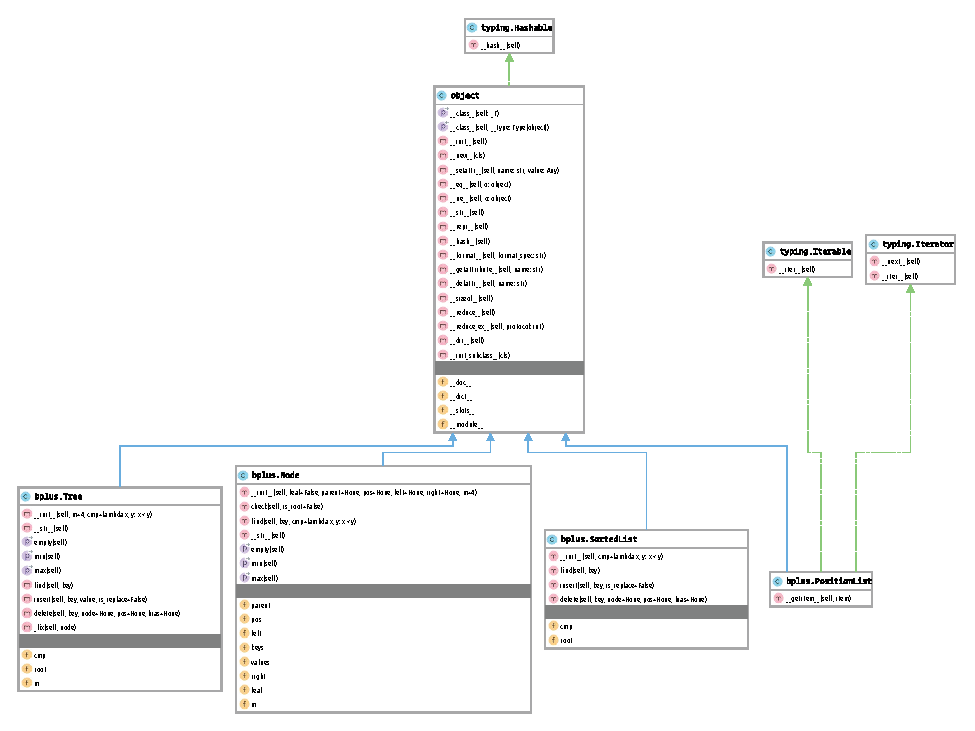
\includegraphics[width=0.85\linewidth]{figure/bplus.eps}
    \caption{B+树的类图与类间关系}
    \label{fig:bplus_diagram}
\end{figure}
\subsection{异常类型}
程序使用的异常类图如\ref{fig:exceptions_diagram}所示。
\begin{figure}[H]
    \centering
    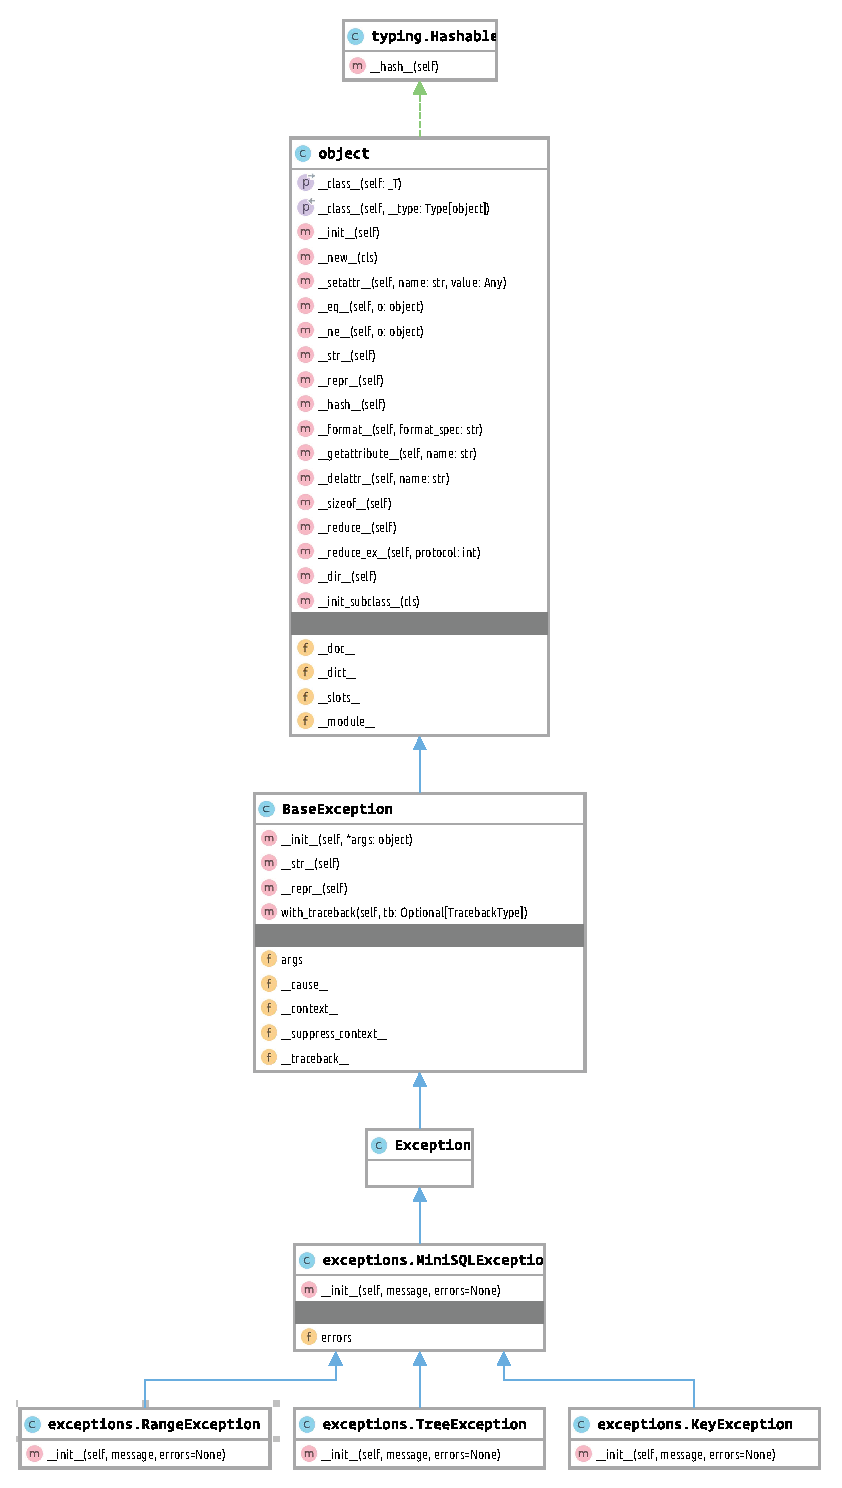
\includegraphics[width=0.5\linewidth]{figure/exceptions.eps}
    \caption{异常的类图与类间关系}
    \label{fig:exceptions_diagram}
\end{figure}
\subsection{索引管理器}
在具体的索引管理器实现上,我们采用了模块层面上的抽象而非类层面的,这更贴合\texttt{Python}语言的风格。
这样能保证尽量大的抽象层次与代码复用率。值得注意的是,我们在实现B+树相关操作的时候也使用了静态函数来抽象部分内容\footnote{我们将在下一部分详细阐述实现细节}。

\chapter{模块实现}
我们通过\texttt{Python}语言来实现各个模块和类。下面我们会通过
\begin{itemize}
    \item 伪代码。
    \item 图表。
    \item 简短的源码。
\end{itemize}
等方式来阐述各个模块的具体实现。

\section{B+树模块具体实现}
\subsection{节点操作具体实现}
节点是B+树中的数据储存元素,每个节点根据要求存储一定数量的排序数据。我们需实首先应实现节点相关操作。算法\ref{alg:binary_searching}实现了一种$O(log\ n)$级别的二分下届查找,用于在某个节点中寻找关键元素。在实际实现中,我们会在C++项目中采用模板,但Python语言的动态类型特性使得这类普适算法很容易应用到具体的数据类型上。
\begin{algorithm}[H]
    \caption{General Binary Search}
    \label{alg:binary_searching}
    \begin{algorithmic}[1]
        \Require The $items$ in iterable list and the $key$ to be searched, optionally the $comparitor$
        \Ensure The $lower_bound$ of the $key$ in $items$, as index
        \Function {BinarySearch}{$items$, $key$, $comparitor=lambda$}
            \State $left \leftarrow 0$
            \State $right \leftarrow \Call{Length}{items}$
            \While{$True$}
                \State $mid \leftarrow (left + right) / 2$
                \If{$left >= right - 1$}
                    \State \textbf{Break}
                \EndIf
                \If{$key < items[mid]$} \Comment{Use custom $comparitor$ if present}
                    \State $right \leftarrow mid$
                \Else
                    \State $left \leftarrow mid$
                \EndIf
            \EndWhile
            \State \Return $mid$
        \EndFunction
    \end{algorithmic}
\end{algorithm}

B+数的查找操作实现如算法\ref{alg:find_on_node}所示,虽然我们正在\textit{节点}模块介绍这一算法,但实际使用中我们往往会通过一颗B+树的根来调用此算法\footnote{本算法会从当前节点开始,一直查询到叶节点。}\footnote{要查找某棵树上的元素,我们只需要从根节点调用此方法。}。

\begin{algorithm}[H]
    \caption{Find Operation on Node}
    \label{alg:find_on_node}
    \begin{algorithmic}[1]
        \Require Current $node$ and the $key$ to be found, optionally the customer $comparitor$
        \Ensure The leaf $node$ and the $position$ of the found element, plus a bias to indicate whether the key is smaller than the smallest element
        \Function{Find}{$node$, $key$, $comparitor=lambda$}
            \State $position \leftarrow \Call{BinarySearch}{node.items, key, comparitor}$
            \If{$position = 0 \cap key < node.keys[0]$}
                \State $bias \leftarrow 0$
            \Else
                \State $bias \leftarrow 1$
            \EndIf
            \If{$\Call{IsLeaf}{node}$}
                \State \Return $\Call{Group}{node, position, bias}$
            \Else
                \State \Return $\Call{Find}{node.children[position + bias], key, comparitor}$
            \EndIf
        \EndFunction
    \end{algorithmic}
\end{algorithm}

\subsection{辅助函数具体实现}
为了方便调用/实现B+树相关功能,并提供代码的抽象程度和复用率,我们使用了一些普适性的函数。例如算法\ref{alg:fix_parent}所示的操作会在节点的头元素修改后修改父节点的相关头元素,如图\ref{fig:fix_parent}所示。
\begin{figure}[H]
    \centering
    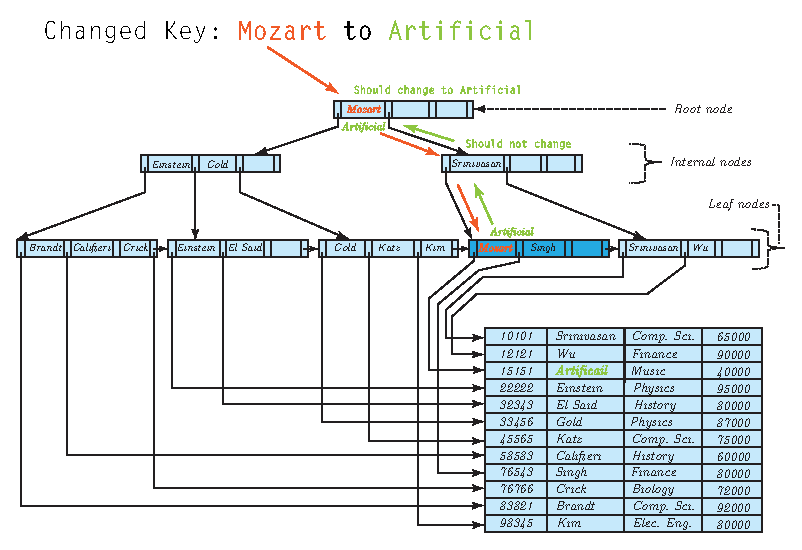
\includegraphics[width=0.8\linewidth]{figure/fix_parent.eps}
    \caption{\texttt{FixParent}}
    \label{fig:fix_parent}
\end{figure}
\begin{algorithm}[H]
    \caption{Fix a Node's Parent After the Left Most Value Is Updated}
    \label{alg:fix_parent}
    \begin{algorithmic}[1]
        \Require The $node$ whose parent is to be fixed
        \Function{FixParent}{$node$}
            \State $key \leftarrow node.keys.front$
            \While{$\Call{Exist}{node.parent} \cap node.position= -1$} \Comment{-1 (position in parent) indicates the node to be the first of parent's children}
                \State $node \leftarrow node.parent$
            \EndWhile
            \If{$\Call{Exist}{node.parent}$}
                \State $node.parent.keys[node.position] \leftarrow key$
            \EndIf
        \EndFunction
    \end{algorithmic}
\end{algorithm}

B+树中节点出现异常\footnote{过饱和,欠饱和等。}后,我们可以直接通过合并节点或拆分节点进行修复操作,也可以首先检查问题节点的姊妹节点是否有修复余地\footnote{有些B+树不会实现这一功能,以降低开发难度。}。本实验中我们采用了首先检查姊妹节点的方式。我们会在进行分裂或合并操作前,检查姊妹是否能否容纳过饱和的冗余或是否有足够多元素为当前问题节点作出补充。
若仍有空余/节点数目足够,则进行修复操作\footnote{对于插入造成的过饱和,删除造成的欠饱和,我们仅仅需要实现一份代码,将问题节点和姊妹节点互换即可复用这一份代码}。此函数的伪代码如算法\ref{alg:fix_sibling}所示,图\ref{fig:fix_sibling}演示了这一过程。

\begin{figure}[H]
    \centering
    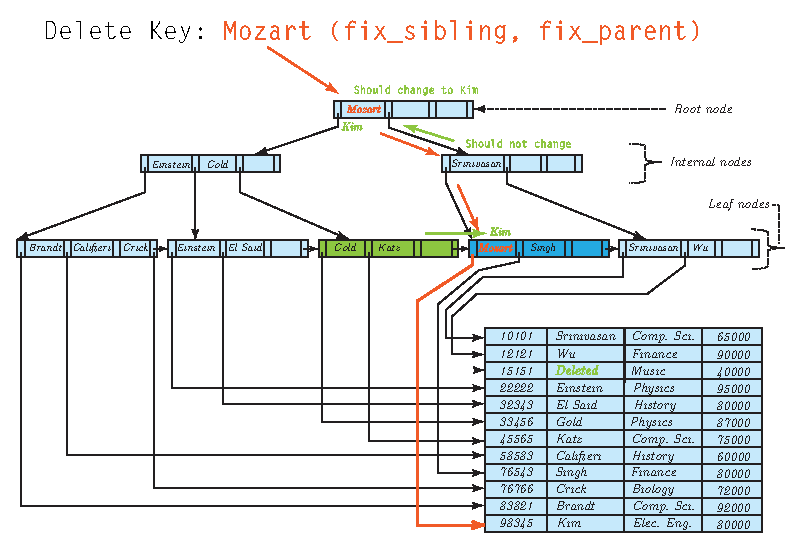
\includegraphics[width=0.8\linewidth]{figure/fix_sibling.eps}
    \caption{\texttt{FixSibling}}
    \label{fig:fix_sibling}
\end{figure}


\begin{algorithm}[H]
    \caption{Fix a Node by Borrowing From a Sibling}
    \label{alg:fix_sibling}
    \begin{algorithmic}[1]
        \Require The $node$ to be fixed
        \Ensure $True$ if fixed, and $False$ if otherwise
        \Function{FixSibling}{$node$}
            \State $sibling \leftarrow node.sibling$ \Comment{next lines will go through both left and right sibling, we'll illustrate the procedure when sibling is left}
            \If{$\Call{Exist}{sibling} \cap \Call{Check}{node}$} \Comment{Check whether node overflows or underflows}
                \State $\Call{MoveValue}{node.keys.front, sibling.keys.back}$ \Comment{Move front of node's keys to end of sibling's keys}
                \State $\Call{MoveValue}{node.values.front, sibling.values.back}$
                \State $\Call{FixParent}{node}$
                \State \Return \textbf{True}
            \Else
                \State \Return \textbf{False}
            \EndIf
        \EndFunction
    \end{algorithmic}
\end{algorithm}

算法\ref{alg:fix_tree}列举了修改在插入或删除操作后出现问题节点的B+树的完整过程\footnote{包含分裂节点与合并节点的具体内容}。它调用了上述的\texttt{FixSibling}和\texttt{FixParent}方法。

\begin{breakablealgorithm}
    \caption{Fix a B+ Tree After Insertion/Deletion}
    \label{alg:fix_tree}
    \begin{algorithmic}[1]
        \Require The $tree$ to be fixed, and the $node$ we've inserted new value on
        \Function{FixTree}{$tree$, $node$}
            \While{True}
                \State $flow \leftarrow \Call{Check}{node}$ \Comment{1 for overflow and -1 for underflow, 0 if node is ok}
                \If{$flow = 0$}
                    \State \textbf{Break}
                \EndIf
                \If{$\Call{FixSibling}{node}$}
                    \State \textbf{Break}
                \EndIf
                \If{$flow = 1$} \Comment{overflow, should split up}
                    \If{$node=tree.root$}
                        \State $tree.root \leftarrow \Call{NewNode}{}$
                        \State $\Call{Append}{tree.children, node}$
                        \State $node.parent \leftarrow tree.root$
                    \EndIf
                    \State $new \leftarrow \Call{NewNode}{}$
                    \If{$\Call{Exist}{new.right}$}
                        \State $new.right.left \leftarrow new$
                        \State $right \leftarrow new.right$
                        \While{$\Call{Exist}{right}$}
                            \State $\Call{Increment}{right.position}$
                            \State $right \leftarrow right.right$
                        \EndWhile
                    \EndIf
                    \State $node.right \leftarrow new$
                    \State $new.keys \leftarrow \Call{LeftHalf}{node.keys}$
                    \State $node.keys \leftarrow \Call{RightHalf}{node.keys}$
                    \State $new.values \leftarrow \Call{LeftHalf}{node.values}$
                    \State $node.values \leftarrow \Call{RightHalf}{node.values}$
                    \State $\Call{Insert}{new.parent.keys, new.position, new.keys.front}$
                    \State $\Call{Insert}{new.parent.children, new.position + 1, new}$
                    \If{$\neg \Call{IsLeaf}{node}$}
                        \State $\Call{Delete}{new.keys.front}$ \Comment{Delete is to delete given element from its container like a Python list}
                    \EndIf
                    \If{$\neg \Call{IsLeaf}{new}$}
                        \For{$child \leftarrow new.children.front$}{$new.children.back$}
                            \State $child.parent \leftarrow new$
                            \State $child.posion \leftarrow index$
                        \EndFor
                    \EndIf
                    \State $node \leftarrow new.parent$ \Comment{Prepare for the next loop, peculate up one level}
                \Else \Comment{underflow, should merge}
                    \If{$\Call{Exist}{node.right}$} \Comment{By default we'd merge current node and its right sibling}
                        \State $node \leftarrow node.left$
                    \EndIf
                    \State $node.keys \leftarrow \Call{Concatenate}{node.keys, node.right.keys}$
                    \State $node.children \leftarrow \Call{Concatenate}{node.children, node.right.children}$
                    \State $\Call{Delete}{node.parent.keys, node.position + 1}$
                    \State $\Call{Delete}{node.parent.children, node.position + 2}$
                    \State $temp \leftarrow node.right$
                    \State $node.right \leftarrow temp.right$
                    \State $\Call{Delete}{temp}$
                    \State $node \leftarrow node.parent$ \Comment{Peculate up one level, prepare for next loop}
                    \If{$node = tree.root$}
                        \State $tree.root = node.children.front$
                        \State $\Call{Delete}{node}$
                    \EndIf
                \EndIf
            \EndWhile
        \EndFunction
    \end{algorithmic}
\end{breakablealgorithm}


\subsection{查询操作具体实现}
详见节点查询部分。
\subsection{插入操作具体实现}
我们通过调用上述的\texttt{Find}与\texttt{FixTree}函数来实现查询操作。具体实现如伪代码\ref{alg:insert_tree}所示。插入等操作具有$\lceil O(\log_{\lceil \frac{m}{2} \rceil}N) \rceil$的时间复杂度。

\begin{algorithm}[H]
    \caption{Insertion in B+ Tree}
    \label{alg:insert_tree}
    \begin{algorithmic}[1]
        \Require The $tree$ object to be inserted into, and the $key$-$value$ pair to be inserted
        \Function{Insert}{$tree$, $key$, $value$}
            \If{$\Call{IsEmpty}{tree}$}
                \State $\Call{Append}{tree.keys, key}$
                \State $\Call{Append}{tree.values, value}$
                \State \Return
            \EndIf
            \State $\Call{Group}{node, position, bias} \leftarrow \Call{Find}{tree.root, key, tree.comparitor}$
            \If{$node.keys[pos] = key$}
                \State \textbf{Raise} $\Call{KeyException}{duplicated\ key}$
            \EndIf
            \State $\Call{Insert}{node.keys, position+bias, key}$
            \State $\Call{Insert}{node.values, position+bias, value}$
            \State $\Call{Fix}{node}$
            \State \Return
        \EndFunction
    \end{algorithmic}
\end{algorithm}

\subsection{删除操作具体实现}
类似插入操纵,我们也会调用上述的\texttt{Find}与\texttt{FixTree}函数来实现B+树中的删除操作。算法\ref{alg:delete_tree}描述了这一过程。


\begin{algorithm}[H]
    \caption{Deletion in B+ Tree}
    \label{alg:delete_tree}
    \begin{algorithmic}
        \Require The $tree$ whose key-value pair is to be deleted, and the $key$ to be deleted
        \Function{Delete}{$tree$, $key$}
            \If{$\Call{Empty}{tree}$}
                \State \textbf{raise} $\Call{TreeException}{Empty\ tree}$
            \EndIf
            \State $\Call{Group}{node, position, bias} \leftarrow \Call{Find}{tree, key}$
            \If{$node.keys[position] \neq key$}
                \State \textbf{raise} $\Call{KeyException}{Cannot\ find\ key}$
            \EndIf
            \State $\Call{Delete}{node.keys[position]}$
            \State $\Call{Delete}{node.children[position]}$ \Comment{On leaf values and keys have the same indices}
            \State $flow \leftarrow \Call{Check}{node}$
            \If{$flow \neq 0$}
                \State $\Call{FixParent}{node}$
            \EndIf
            \State $\Call{FixTree}{tree, node}$
        \EndFunction
    \end{algorithmic}
\end{algorithm}

\section{异常模块具体实现}
我们通过异常机制来传递错误信息,省去了检测错误码的冗长代码。实验中B+树和索引管理器模块用到的异常如列表\ref{lst:exception}所示。

\begin{longlisting}
\begin{minted}{python}
class MiniSQLException(Exception):
    """
    raised when we cannot find a particular key
    or duplication occurs
    """

    def __init__(self, message, errors=None):
        # Call the base class constructor with the parameters it needs
        super().__init__(message)

        # Now for your custom code...
        self.errors = errors


class KeyException(MiniSQLException):
    def __init__(self, message, errors=None):
        super().__init__(message, errors)


class RangeException(MiniSQLException):
    def __init__(self, message, errors=None):
        super().__init__(message, errors)


class TreeException(MiniSQLException):
    def __init__(self, message, errors=None):
        super().__init__(message, errors)
\end{minted}
\caption{异常类型的具体实现}
\label{lst:exception}
\end{longlisting}

\section{备用数据结构具体实现}
为了满足特殊操作\footnote{如,要求插入的键值对中\textbf{值}永远是当前的下标。}我们实现了一种特殊的数据结构:\textit{排序数组索引结构},其具备了如下特点:
\begin{itemize}
    \item 查询操作时间同样为$O(log\ N)$。
    \item 进行各项其他操作表现如同数组,没有冗杂的数据结构与算法支撑。
    \item 提供与B+树完全相同的接口。
\end{itemize}
其具体实现和算法\ref{alg:binary_searching},\ref{alg:find_on_node}以及\ref{alg:insert_tree}描述的很相似,只不过去除了复杂的修复部分。我们通过图\ref{fig:sorted_list}来进一步描述这一过程\footnote{若插图过小请放大,我们使用了矢量图。}。

\begin{figure}[H]
    \centering
    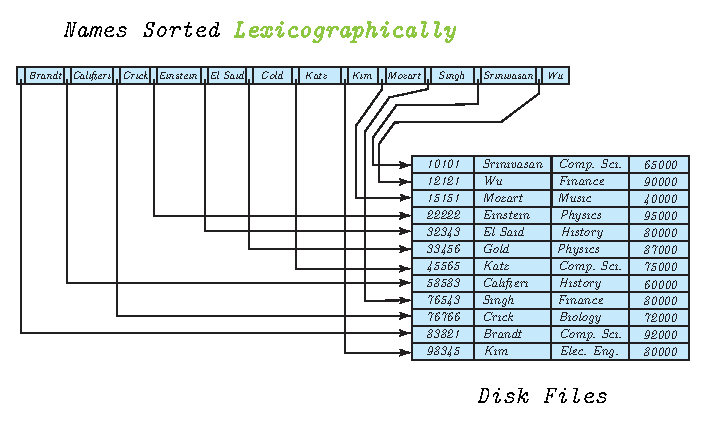
\includegraphics[width=0.5\linewidth]{figure/sorted_list.eps}
    \caption{排序数组具体实现}
    \label{fig:sorted_list}
\end{figure}


\section{索引管理器模块具体实现}
我们根据索引管理器系统的要求实现了逻辑管理器模块,并进行了一定程度上的逻辑抽象和代码复用。

\subsection{整体索引操作}
对完整索引进行的操作如算法\ref{alg:index_creation_deletion}所示。

\algnewcommand\algorithmicraise{\textbf{raise}}
\algnewcommand\Raise{\item[\algorithmicraise]}

\begin{algorithm}
    \caption{索引的插入删除}
    \label{alg:index_creation_deletion}
    \begin{algorithmic}
        \Function{CreateIndex}{$data\_list$, $comparitor$}
            \State $tree \leftarrow \Call{NewTree}{comparitor}$
            \ForAll{$data \in data\_list$}
                \State $\Call{InsertTree}{tree, data[i]}$
            \EndFor
            \State $\Call{SaveBufferIndex}{tree}$
        \EndFunction
        \Function{DropIndex}{$id$}
            \State $\Call{DropBufferIndex}{id}$
        \EndFunction
    \end{algorithmic}
\end{algorithm}

\subsection{元素寻找,插入,删除具体实现}

\begin{algorithm}
    \caption{元素的插入,删除和删除}
    \begin{algorithmic}
        \Function{InsertElement}{$id$, $key$, $value$}
            \State $tree \leftarrow \Call{GetBufferIndex}{id}$
            \State $\Call{InsertTree}{tree, key, value}$
            \State $\Call{SaveBufferIndex}{tree, ind}$ \Comment{Specify the id, so that buffer manager can replace}
        \EndFunction
    \end{algorithmic}
\end{algorithm}


\chapter{遇到的问题及解决方法}
\chapter{总结}

\newpage
\part{附录}


\begin{appendices}
\chapter{接口说明}

\chapter{插图,表格与列表}
\listoffigures
\listoftables
\listoflistings
\end{appendices}
\end{document}